\documentclass{beamer}

% xcolor and define colors -------------------------
\usepackage{xcolor}

% https://www.viget.com/articles/color-contrast/
\definecolor{purple}{HTML}{5601A4}
\definecolor{navy}{HTML}{0D3D56}
\definecolor{ruby}{HTML}{9a2515}
\definecolor{alice}{HTML}{107895}
\definecolor{daisy}{HTML}{EBC944}
\definecolor{coral}{HTML}{F26D21}
\definecolor{kelly}{HTML}{829356}
\definecolor{cranberry}{HTML}{E64173}
\definecolor{jet}{HTML}{131516}
\definecolor{asher}{HTML}{555F61}
\definecolor{slate}{HTML}{314F4F}

% Mixtape Sessions
\definecolor{picton-blue}{HTML}{00b7ff}
\definecolor{violet-red}{HTML}{ff3881}
\definecolor{sun}{HTML}{ffaf18}
\definecolor{electric-violet}{HTML}{871EFF}

% Main theme colors
\definecolor{accent}{HTML}{00b7ff}
\definecolor{accent2}{HTML}{871EFF}
\definecolor{gray100}{HTML}{f3f4f6}
\definecolor{gray800}{HTML}{1F292D}


% Beamer Options -------------------------------------

% Background
\setbeamercolor{background canvas}{bg = white}

% Change text margins
\setbeamersize{text margin left = 15pt, text margin right = 15pt} 

% \alert
\setbeamercolor{alerted text}{fg = accent2}

% Frame title
\setbeamercolor{frametitle}{bg = white, fg = jet}
\setbeamercolor{framesubtitle}{bg = white, fg = accent}
\setbeamerfont{framesubtitle}{size = \small, shape = \itshape}

% Block
\setbeamercolor{block title}{fg = white, bg = accent2}
\setbeamercolor{block body}{fg = gray800, bg = gray100}

% Title page
\setbeamercolor{title}{fg = gray800}
\setbeamercolor{subtitle}{fg = accent}

%% Custom \maketitle and \titlepage
\setbeamertemplate{title page}
{
    %\begin{centering}
        \vspace{20mm}
        {\Large \usebeamerfont{title}\usebeamercolor[fg]{title}\inserttitle}\\
        {\large \itshape \usebeamerfont{subtitle}\usebeamercolor[fg]{subtitle}\insertsubtitle}\\ \vspace{10mm}
        {\insertauthor}\\
        {\color{asher}\small{\insertdate}}\\
    %\end{centering}
}

% Table of Contents
\setbeamercolor{section in toc}{fg = accent!70!jet}
\setbeamercolor{subsection in toc}{fg = jet}

% Button 
\setbeamercolor{button}{bg = accent}

% Remove navigation symbols
\setbeamertemplate{navigation symbols}{}

% Table and Figure captions
\setbeamercolor{caption}{fg=jet!70!white}
\setbeamercolor{caption name}{fg=jet}
\setbeamerfont{caption name}{shape = \itshape}

% Bullet points

%% Fix left-margins
\settowidth{\leftmargini}{\usebeamertemplate{itemize item}}
\addtolength{\leftmargini}{\labelsep}

%% enumerate item color
\setbeamercolor{enumerate item}{fg = accent}
\setbeamerfont{enumerate item}{size = \small}
\setbeamertemplate{enumerate item}{\insertenumlabel.}

%% itemize
\setbeamercolor{itemize item}{fg = accent!70!white}
\setbeamerfont{itemize item}{size = \small}
\setbeamertemplate{itemize item}[circle]

%% right arrow for subitems
\setbeamercolor{itemize subitem}{fg = accent!60!white}
\setbeamerfont{itemize subitem}{size = \small}
\setbeamertemplate{itemize subitem}{$\rightarrow$}

\setbeamertemplate{itemize subsubitem}[square]
\setbeamercolor{itemize subsubitem}{fg = jet}
\setbeamerfont{itemize subsubitem}{size = \small}


% Special characters

\usepackage{collectbox}

\makeatletter
\newcommand{\mybox}{%
    \collectbox{%
        \setlength{\fboxsep}{1pt}%
        \fbox{\BOXCONTENT}%
    }%
}
\makeatother





% Links ----------------------------------------------

\usepackage{hyperref}
\hypersetup{
  colorlinks = true,
  linkcolor = accent2,
  filecolor = accent2,
  urlcolor = accent2,
  citecolor = accent2,
}


% Line spacing --------------------------------------
\usepackage{setspace}
\setstretch{1.1}


% \begin{columns} -----------------------------------
\usepackage{multicol}


% Fonts ---------------------------------------------
% Beamer Option to use custom fonts
\usefonttheme{professionalfonts}

% \usepackage[utopia, smallerops, varg]{newtxmath}
% \usepackage{utopia}
\usepackage[sfdefault,light]{roboto}

% Small adjustments to text kerning
\usepackage{microtype}



% Remove annoying over-full box warnings -----------
\vfuzz2pt 
\hfuzz2pt


% Table of Contents with Sections
\setbeamerfont{myTOC}{series=\bfseries, size=\Large}
\AtBeginSection[]{
        \frame{
            \frametitle{Roadmap}
            \tableofcontents[current]   
        }
    }


% Tables -------------------------------------------
% Tables too big
% \begin{adjustbox}{width = 1.2\textwidth, center}
\usepackage{adjustbox}
\usepackage{array}
\usepackage{threeparttable, booktabs, adjustbox}
    
% Fix \input with tables
% \input fails when \\ is at end of external .tex file
\makeatletter
\let\input\@@input
\makeatother

% Tables too narrow
% \begin{tabularx}{\linewidth}{cols}
% col-types: X - center, L - left, R -right
% Relative scale: >{\hsize=.8\hsize}X/L/R
\usepackage{tabularx}
\newcolumntype{L}{>{\raggedright\arraybackslash}X}
\newcolumntype{R}{>{\raggedleft\arraybackslash}X}
\newcolumntype{C}{>{\centering\arraybackslash}X}

% Figures

% \imageframe{img_name} -----------------------------
% from https://github.com/mattjetwell/cousteau
\newcommand{\imageframe}[1]{%
    \begin{frame}[plain]
        \begin{tikzpicture}[remember picture, overlay]
            \node[at = (current page.center), xshift = 0cm] (cover) {%
                \includegraphics[keepaspectratio, width=\paperwidth, height=\paperheight]{#1}
            };
        \end{tikzpicture}
    \end{frame}%
}

% subfigures
\usepackage{subfigure}


% Highlight slide -----------------------------------
% \begin{transitionframe} Text \end{transitionframe}
% from paulgp's beamer tips
\newenvironment{transitionframe}{
    \setbeamercolor{background canvas}{bg=accent!40!black}
    \begin{frame}\color{accent!10!white}\LARGE\centering
}{
    \end{frame}
}


% Table Highlighting --------------------------------
% Create top-left and bottom-right markets in tabular cells with a unique matching id and these commands will outline those cells
\usepackage[beamer,customcolors]{hf-tikz}
\usetikzlibrary{calc}
\usetikzlibrary{fit,shapes.misc}

% To set the hypothesis highlighting boxes red.
\newcommand\marktopleft[1]{%
    \tikz[overlay,remember picture] 
        \node (marker-#1-a) at (0,1.5ex) {};%
}
\newcommand\markbottomright[1]{%
    \tikz[overlay,remember picture] 
        \node (marker-#1-b) at (0,0) {};%
    \tikz[accent!80!jet, ultra thick, overlay, remember picture, inner sep=4pt]
        \node[draw, rectangle, fit=(marker-#1-a.center) (marker-#1-b.center)] {};%
}

\usepackage{breqn} % Breaks lines

\usepackage{amsmath}
\usepackage{mathtools}

\usepackage{pdfpages} % \includepdf

\usepackage{listings} % R code
\usepackage{verbatim} % verbatim

% Video stuff
\usepackage{media9}

% packages for bibs and cites
\usepackage{natbib}
\usepackage{har2nat}
\newcommand{\possessivecite}[1]{\citeauthor{#1}'s \citeyearpar{#1}}
\usepackage{breakcites}
\usepackage{alltt}

% Setup math operators
\DeclareMathOperator{\E}{E} \DeclareMathOperator{\tr}{tr} \DeclareMathOperator{\se}{se} \DeclareMathOperator{\I}{I} \DeclareMathOperator{\sign}{sign} \DeclareMathOperator{\supp}{supp} \DeclareMathOperator{\plim}{plim}
\DeclareMathOperator*{\dlim}{\mathnormal{d}\mkern2mu-lim}
\newcommand\independent{\protect\mathpalette{\protect\independenT}{\perp}}
   \def\independenT#1#2{\mathrel{\rlap{$#1#2$}\mkern2mu{#1#2}}}
\newcommand*\colvec[1]{\begin{pmatrix}#1\end{pmatrix}}

\newcommand{\myurlshort}[2]{\href{#1}{\textcolor{gray}{\textsf{#2}}}}


\begin{document}

\imageframe{./lecture_includes/mixtape_did_cover.png}


% ---- Content ----



\section{Conditional Parallel Trends}

\subsection{Introducing Covariates}

\begin{frame}{Review}

\begin{itemize}
\item Diff in Diff is a quasi-experimental method that identifies the aggregate causal parameter, ATT, if:

	\begin{enumerate}
	\item Parallel trends holds
	\item And also no anticipation and if we use comparisons that aren't treated
	\end{enumerate}
	
\item But we worked with "unconditional parallel trends" which means this:

	$$ \bigg ( \textcolor{red}{E[Y^0_k|Post]} - E[Y^0_k|Pre] \bigg ) - \bigg ( E[Y^0_U|Post] - E[Y^0_U | Pre] \bigg )$$
	
\item This means that the \emph{average} treatment group potential outcome trends for our treatment group is the same as our control group

\end{itemize}

\end{frame}

\begin{frame}{Is Unconditional Parallel Trends Plausible?}

\begin{itemize}

\item But what if these two groups are different in ways that predict $Y^0$?

\item Let's say for instance that your study looks at an intervention that primarily effects cities, but your only control group are rural counties

\item These groups differ in a ways that might, depending on your study, not be plausibly suggesting they would've been on the same trends

\end{itemize}

\end{frame}

\begin{frame}{Conditional parallel trends}

\begin{itemize}

\item While it isn't required that two groups -- group $k$ and group $U$ -- be similar on observables for parallel trends to hold:

	\begin{enumerate}
	\item Remember, if treatment had been random, then they would have the average covariates
	\item And if they aren't, then you may need to provide more evidence that these differences are irrelevant
	\item So you should still check and see and if they aren't, you either adjust or have a good justification for why they're the same on trends in $E[Y^0]$ 
	\end{enumerate}
	
\item Including covariates weakens the unconditional parallel trends assumption by only requiring that units with similar covariate values, as opposed to everyone, follow similar counterfactual trends in $Y^0$
\item This is means switching out the \emph{unconditional parallel trends} assumption for the \emph{conditional parallel trends} assumption

\end{itemize}

\end{frame}

\begin{frame}{Why covariates?}

\begin{itemize}

\item The inclusion of covariates in diff-in-diff models is not about trying to find random variation in the treatment within values of the dimension of X
\item It is based on the claim that the inclusion of covariates is necessary to re-establish parallel trends
\item This is itself different than how covariates will be used in synthetic control, too
\end{itemize}

\end{frame}




\begin{frame}{Correcting the missingness problem}

\begin{eqnarray*}
\text{ATT} &=& E[\delta | D=1] \\
&=& E[Y^1-\textcolor{red}{Y^0} | D=1] \\
&=& E[Y^1 | D=1] - \textcolor{red}{E[Y^0|D=1]} \\
&=& E[Y | D=1] - \textcolor{red}{E[Y^0|D=1]} 
\end{eqnarray*}

\bigskip

We were always missing $Y^0$ values for the treatment group units, but parallel trends allowed us to impute it using the change in $[Y^0]|D=0]$ as a guide

\bigskip

But if that trend is not a good guide, then we cannot.  


\end{frame}


\begin{frame}{Conditional parallel trends}

The DiD equation yields:

\begin{eqnarray*}
\widehat{\delta} &=& \bigg ( E[Y_k|Post] - E[Y_k|Pre] \bigg ) - \bigg ( E[Y_U | Post ] - E[ Y_U | Pre] \bigg) \\
&=& \text{ATT} + \text{Non-parallel trends bias}
\end{eqnarray*}

\bigskip

If we believe that conditional on covariates, parallel trends holds, but only within values of $X$, then there are methods we can use that incorporate covariates into the DiD equation and unbiasedness returns

\bigskip 

The inclusion of covariates has particular regression specifications, plus there are alternative methods too, and we will review them

\end{frame}

\subsection{Choosing Covariates}

\begin{frame}{Picking covariates}

\begin{itemize}
\item You want to select confounders, which are baseline untreated covariates that predict both the treatment (and thus cause imbalance) but also the potential outcome, $Y^0$
\item You can use your common sense, logic, graphical models (i.e., DAGs) and familiarity of the subject 
	\begin{itemize}
	\item Our focus is on the covariates that are determinants of the outcome, and less so the treatment itself, because note our concern is the untreated potential outcome $Y^0$
	\end{itemize}
\item But you can also use some simple approaches that I'll suggest now
\end{itemize}

\end{frame}

\begin{frame}{Three ideas}

\begin{itemize}
\item Note that we are missing $\textcolor{red}{E[Y^0|D=1]}$, and so we want covariates that are highly predictive of that missing potential outcome -- problem is, it's missing
\item But what if we did this:
	\begin{enumerate}
	\item Drop all treated (post treatment treatment group) so that all outcomes are now $Y^0$ and regress that against candidate covariates, and select from there
	\item Drop post treatment treatment group units and drop the control units and regress $Y^0$ for the treated unit against baseline covariates and select from there
	\item Use $t-2$ and $t-1$ period, calculate $\Delta E[Y^0|D=1]$ and regress that against $t-1$ covariates and select from there
	\end{enumerate}
\item This is a more data driven procedure and is helping you figure out which covariates might be candidate confounders -- but note this still is not checking for imbalance
\end{itemize}

\end{frame}


\subsection{Checking for Imbalance}

\begin{frame}
    \frametitle{Covariate Balance and Parallel Trends}
    \begin{itemize}
        \item The parallel trends assumption is untestable but can be evaluated using observed covariates.
        \item Balance in key covariates helps assess whether treated and control groups would follow similar trends.
        \item Differences in demographics or economic conditions between groups can indicate violations of parallel trends.
        \item Use covariates that are unlikely to be affected by treatment to check balance.
    \end{itemize}
\end{frame}


\begin{frame}
    \frametitle{Baseline Covariates and Normalized Difference}
    \begin{itemize}
        \item Baseline covariates are measured before treatment ($t-1$). Check for balance between treatment and control groups.
        \item Report the averages of covariates for both groups in a table.
        \item The normalized difference is calculated as:
        $$ \text{Norm. Diff}_\omega = \frac{\overline{X}_{\omega,T} - \overline{X}_{\omega,C}}{\sqrt{(S_{\omega,T}^2 + S_{\omega,C}^2)/2}} $$
        \item The normalized difference measures imbalance; it should be less than 0.25 to avoid problematic imbalance Imbens and Rubin (2015).
    \end{itemize}
\end{frame}


\begin{frame}{Normalized Difference vs. Z-Score}
    \begin{itemize}
        \item \textbf{Normalized Difference:}
        \begin{itemize}
            \item Measures difference in group means (e.g., treatment vs. control)
            \item Interprets difference relative to pooled variance
            \item Used for comparing balance between groups
        \end{itemize}
        \vspace{0.5em}
        \item \textbf{Z-Score:}
        \begin{itemize}
            \item Measures distance of a single observation from the mean
            \item Expresses this distance in standard deviation units
            \item Used for assessing how unusual a single observation is
        \end{itemize}
        \vspace{0.5em}
        \item Both metrics standardize differences using standard deviation, making them unit-free and comparable across variables, but in our case we need to focus on differences between two groups, so we use the normalized difference and focus on a threshold of 0.25.
    \end{itemize}
\end{frame}


\begin{frame}
    \centering
    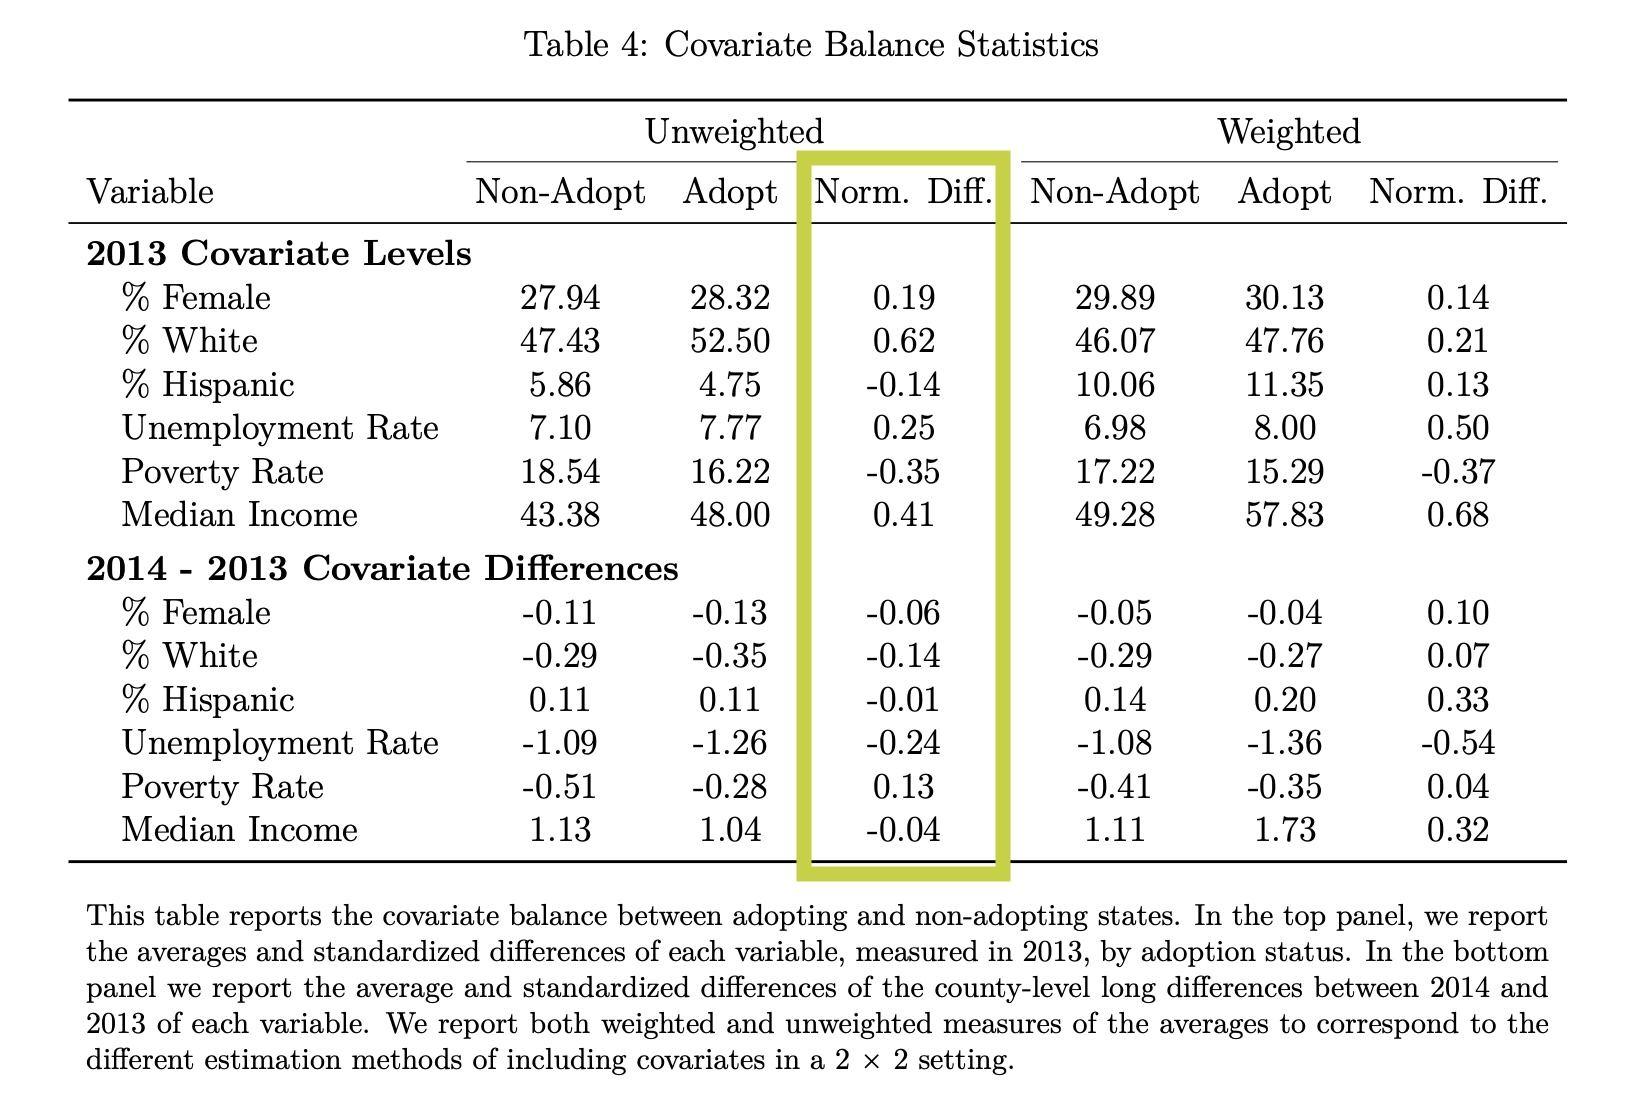
\includegraphics[width=0.9\textwidth]{./lecture_includes/table_jel_covariates.jpg}
\end{frame}

\begin{frame}
    \frametitle{Intuition for Checking Covariate Balance}
    \begin{itemize}
    \item Remember that confounders are variables that do two things
    	\begin{enumerate}
	\item $X \rightarrow D$. Confounders have different distributions in treatment than control and these balance checks are about seeing if that's true
	\item $X \rightarrow \Delta E[Y^0]$. But it's only a problem if the imbalance is on variables that also predict potential outcome trends, and we choose covariates based on things we think that's true
	\end{enumerate}
\item So you select covariates that you think are theoretically predictive of $Y^0$ trends, but then you check imbalance to see if they are differentially distributed 
    \end{itemize}
\end{frame}


\begin{frame}{Example: Murder}

\begin{itemize}
\item Say that there a set of cities pass gun law ordinances but smaller towns don't and you want to know its effect on homicides
\item Maybe as much as 80\% of homicides are in cities -- the homicides in small towns are rare, and the trends are probably pretty noisy and different
\item So you might think population size, could be a very important covariate to include or urbanization
\end{itemize}

\end{frame}





\begin{frame}{Three covariate DiD papers}

Three papers (though sometimes you see others) about covariate adjustment in DiD:
\begin{enumerate}
\item Abadie (2005) on semiparametric DiD -- reweights the comparison group part of the DID equation using a propensity score based on X
\item Heckman, Ichimura and Todd (1997) on outcome regression uses baseline X and control group only to impute the missing counterfactual $Y^0$ for treatment group units in a DiD equation
\item Sant'Anna and Zhou (2020) is double robust which means the method does both of these at the same time so that you don't have to choose between them
\end{enumerate}

\bigskip

We will discuss both of them and then compare their performance with the more straightforward fixed effects model

\end{frame}


\section{Estimators}

\subsection{Inverse probability weighting}




\begin{frame}{Semiparametric DiD}


 Abadie (2005) proposed a model that simply reweights the control group in the DiD equation using a particular specification (``semiparametric'') of the propensity score on pretreatment covariates
 
	\begin{enumerate}
	\item Calculate each unit's ``after minus before'' (DiD equation)
	\item Estimate the conditional probability of treatment based on baseline covariates (propensity score estimation)
	\item Weight the comparison group's DiD equation with the propensity score 
	\end{enumerate}

Remember -- ATT is only missing $Y^0$ for treatment, so we only have to apply weights to the comparison group units

\end{frame}

\begin{frame}{Novel elements of time in Abadie's model}

\begin{itemize}
\item There is only one treatment group so therefore there is only one relevant treatment date, $t$
\item The period prior to treatment is called the baseline, or $b$, period and it is when treated units were not treated 
\item $X_b$ are ``baseline'' covariates meaning the value of $X$ in the pre-treatment period for either the treated or comparison group units
\item Propensity scores are estimated off the $b$ period \emph{only} 
\item Abadie ``throws away'' covariates after treatment because this is all about re-establishing parallel trends which is a \emph{baseline} concept recall
\end{itemize}

\end{frame}

\begin{frame}{Assumptions}

Five main assumptions

\begin{enumerate}
\item No anticipation 
\item SUTVA
\item Conditional parallel trends $$E[Y^0_t - Y^0_b|D=1,X_b] = E[Y^0_t - Y^0_t | D=0, X_b]$$ 
\item Common support $$Pr(D=1)>0; Pr(D=1|X)<1$$ 
\item Propensity score model is properly specified 
\end{enumerate}

\end{frame}

\begin{frame}{Propensity scores as dimension reduction}

\begin{itemize}

\item Propensity scores are ways of dealing with a conditioning set $X$ that has large dimensions
\item Dimensions are not the same as covariates -- if you have continuous $X$, then it has infinite dimensions
\item Common support means that \emph{within} all combinations of the covariates (e.g., white male 47yo versus whites, males, age) there are units in treatment and control

\end{itemize}

\end{frame}

\begin{frame}{Common support example}

Think of common support like ``exact matches'' but on the propensity score

\bigskip

I'm a white male 47 years old with a PhD; can I find a white male 47 years old without a PhD

\bigskip

If I can, that's common support; if I cannot that's off support

\end{frame}


\begin{frame}{Propensity scores as dimension reduction}

\begin{itemize}

\item Propensity score theorem (Rosenbaum and Rubin 1983) showed that if you need $X$ to satisfy some assumption, the propensity score will satisfy too
\item Propensity scores essentially transform your large dimensional problem into a single scalar called the propensity score, which is the conditional probability of treatment (conditional on $X$)
\item But we need to estimate the propensity score because we don't usually know it (only an experimentalist ``knows'' the true propensity score)

\end{itemize}

\end{frame}

\begin{frame}{Common support and the propensity score}

\begin{itemize}
\item Exact matches mean you have people who are identical on covariate values in both treatment and control
\item Common support and the propensity score means you have people nearly identical on their probability of treatment
\item I am 47yo white male with a PhD with a propensity score of 0.75, but you are an Asian female 27yo without a PhD and have a propensity score of 0.75
\item Same idea, but for this to work, we need to have ``matches'' like that (just on the propensity score)
\end{itemize}

\end{frame}


\begin{frame}{How do these work together?}

Since we are identifying the ATT, and the ATT is missing $Y^0$ for the treated group, we are using the control group $Y^0$ in its place 

\bigskip

Under conditional parallel trends and common support, some of the comparison group units are recovering the parallel trends because of their $X$ values creating projections that in their differences perfectly aligned in expectation with the missing $\Delta E[Y^0|D=1]$

\bigskip

But we have to have all three for it to work

\end{frame}

\begin{frame}{Visualizing propensity score to get common support}

	\begin{figure}
	\includegraphics[scale=0.05]{./lecture_includes/common_support_abadie.png}
	\end{figure}

\end{frame}

\begin{frame}{Definition and estimation}

Defining the ATT parameter of interest
\begin{eqnarray*}
ATT &=& E[Y^1_t - \textcolor{red}{Y^0_t} |D=1] \\
&=&E[Y^1_t  | D = 1 ] - \textcolor{red}{E[Y^0_t | D=1]}
\end{eqnarray*}

\bigskip
Abadie's inverse probability weighting (IPW) estimator
\begin{eqnarray*}
E\bigg [ \frac{Y_t - Y_b}{Pr(D_t=1)} \times \frac{D_t - Pr(D=1|X_b)}{1-Pr(D=1|X_b)} \bigg ]
\end{eqnarray*}

\bigskip

The first is our causal parameter; the second is our reweighted DiD equation that \emph{estimates} our causal parameter, but we need to estimate that propensity score


\end{frame}

\begin{frame}{Abadie's IPW estimator}

Look closely; what happens mathematically when you substitute $D=1$ vs $D=0$?

\begin{eqnarray*}
E\bigg [ \frac{Y_t - Y_b}{Pr(D_t=1)} \times \frac{D_t - Pr(D=1|X_b)}{1-Pr(D=1|X_b)} \bigg ]
\end{eqnarray*}

\bigskip

The reweighting with the propensity only happens to the comparison group's first differences -- not the treatment groups!  Why?  Because it's the $Y^0$ that is missing, not the $Y^1$

\end{frame}



\begin{frame}{Propensity scores}

\begin{itemize}
\item It's common to hear people say that we don't know the propensity score; we can only estimate it. Same here -- we approximate it with regressions
\item Paper is titled ``Semi-parametric DiD'' because Abadie imposes structure on the polynomials used to construct the propensity score (``series logit'')
\end{itemize}

\end{frame}



\begin{frame}{Abadie 2005 influence}

	\begin{figure}
	\includegraphics[scale=0.25]{./lecture_includes/abadie_restud_ipw}
	\end{figure}Abadie (2005) is his fourth most cited paper

\end{frame}




\subsection{Outcome Regression and Canonical OLS with Additive Controls}



\begin{frame}{Doubly Robust Difference-in-differences}

\begin{itemize}
\item DR models control for covariates twice -- once using the propensity score, once using outcomes adjusted by regression -- and are unbiased so long as:
	\begin{itemize}
	\item The regression specification for the outcome is correctly specified
	\item The propensity score specification is correctly specified
	\end{itemize}
\item Sant'Anna and Zhao (2020) incorporated DR into DiD by combining inverse probability weighting and outcome regression into a single DiD model
\item It's in the engine of Callaway and Sant'Anna (2020) that we discuss later so it merits close study
\end{itemize}

\end{frame}




\begin{frame}{Identification assumptions I: Data}

Assumption 1: Assume panel data or repeated cross-sectional data

\bigskip

Handling repeated cross-sectional data is possible but assumes stationarity which is a kind of stability assumption, but I'll use panel representation. 

\bigskip

Cross-sections will be potentially violated with changing sample compositions (e.g., the Napster example). 

\end{frame}

\begin{frame}{Identification assumptions II: Modification to parallel trends}

Assumption 2: Conditional parallel trends

\bigskip

Counterfactual trends for the treatment group are the same as the control group for all values of $X$

\begin{eqnarray*}
E[Y_1^0 - Y_0^0 | X, D=1] = E[Y^0_1 - Y^0_0 | X, D=0]
\end{eqnarray*}

\end{frame}

\begin{frame}{Identification assumptions III: Common support}

Assumption 3: Common support

\bigskip

For some $e>0$, the probability of being in the treatment group is greater than $e$ and the probability of being in the treatment group conditional on $X$ is $\leq1-e$. 

\bigskip

Heckman, et al doesn't use the propensity score so we need a more general expression of support

\end{frame}

\begin{frame}{Estimating DD with Assumptions 1-3}

\begin{itemize}
\item Assumptions 1-3 gives us a couple of options of estimating the DiD
\item We can either use the outcome regression (OR) approach of Heckman, et al 1997 (will require correct model too)
\item Or we can use the inverse probability weighting (IPW) approach of Abadie (2005) (will require correct model too)
\end{itemize}

\end{frame}



\begin{frame}{Outcome regression}

This is the Heckman, et al. (1997) approach where the potential outcome evolution for the treatment group is imputed with a regression based only on $X_b$ for the control group \emph{only}

\bigskip

\begin{eqnarray*}
\widehat{\delta}^{OR} = \overline{Y}_{1,1} - \bigg [ \overline{Y}_{1,0} + \frac{1}{n^T} \sum_{i|D_i=1} ( \widehat{\mu}_{0,1}(X_i) - \widehat{\mu}_{0,0}(X_i)) \bigg ]
\end{eqnarray*}

where $\overline{Y}$ is the sample average of $Y$ among units in the treatment group at time $t$ and $\widehat{\mu}(X)$ is an estimator of the true, but unknown, $m_{d,t}(X)$ which is by definition equal to $E[Y_t|D=d,X=x]$.

\end{frame}




\begin{frame}{Outcome regression}

\begin{eqnarray*}
\widehat{\delta}^{OR} = \overline{Y}_{1,1} - \bigg [ \overline{Y}_{1,0} + \frac{1}{n^T} \sum_{i|D_i=1} ( \widehat{\mu}_{0,1}(X_i) - \widehat{\mu}_{0,0}(X_i)) \bigg ]
\end{eqnarray*}

\begin{enumerate}
\item Regress changes $\Delta Y$ on $X$ among untreated groups using baseline covariates only
\item Get fitted values of the regression using all $X$ from $D=1$ only.  Average those
\item Calculate change in this fitted $Y$ among treated with the average fitted values
\end{enumerate}

\end{frame}

\begin{frame}{Inverse probability weighting}

This is the Abadie (2005) approach where we use weighting

\begin{eqnarray*}
\widehat{\delta}^{ipw} = \frac{1}{E_N[D]} E \bigg [ \frac{D-\widehat{p}(X)}{1-\widehat{p}(X)} (Y_1-Y_0) \bigg ]
\end{eqnarray*}

where $\widehat{p}(X)$ is an estimator for the true propensity score. Reduces the dimensionality of $X$ into a single scalar.

\end{frame}

\begin{frame}{These models cannot be ranked}

\begin{itemize}
\item Outcome regression needs $\widehat{\mu}(X)$ to be correctly specified, whereas
\item Inverse probability weighting needs $\widehat{p}(X)$ to be correctly specified
\item It's hard to ``rank'' these two in practice with regards to model misspecification because each is inconsistent when their own models are misspecified
\item But what if you could do both of them at the same time and not pay for it?
\end{itemize}

\end{frame}

\begin{frame}{Double Robust DR}

\begin{itemize}
\item Doubly robust combines them to give us insurance; we now get two chances to be wrong, as opposed to just one
\item Two papers:
	\begin{enumerate}
	\item Chang (2020) incorporates DR with double/debiased ML
	\item Sant'Anna and Zhau (2020) is based on the IPW (Abadie 2005) and OR (Heckman, Ichimura and Todd 1997)
	\end{enumerate}
\item For now, I've prepped the latter, but will soon get Chang (2020) incorporated -- I just have been relying on Brigham Frandsen to teach the DML material
\end{itemize}

\end{frame}


\subsection{Double Robust}

\begin{frame}{Double Robust DiD}
\begin{eqnarray*}
\delta^{dr} = E \bigg [ \bigg ( \frac{D}{E[D]} -\frac{ \frac{p(X)(1-D)}{(1-p(X))} }{E \bigg [\frac{p(X)(1-D)}{(1-p(X))} \bigg ]} \bigg  )( \Delta Y - \mu_{0,\Delta}(X)) \bigg ]
\end{eqnarray*}

\begin{eqnarray*}
&&p(x): \text{propensity score model} \\
&& \Delta Y = Y_1 - Y_0 = Y_{post} - Y_{pre} \\
&& \mu_{d,\Delta} = \mu_{d,1}(X) - \mu_{d,0}(X), \text{ where } \mu(X) \text{ is a model for} \\
&& m_{d,t} = E[Y_t|D=d,X=x]
\end{eqnarray*}So that means $\mu_{0,\Delta}$ is just the control group's change in average $Y$ for each $X=x$

\end{frame}

\begin{frame}{Double Robust DiD}

\begin{eqnarray*}
\delta^{dr} = E \bigg [ \bigg ( \frac{D}{E[D]} -\frac{ \frac{p(X)(1-D)}{(1-p(X))} }{E \bigg [\frac{p(X)(1-D)}{(1-p(X))} \bigg ]} \bigg  )( \Delta Y - \mu_{0,\Delta}(X)) \bigg ]
\end{eqnarray*}

Notice how the model controls for $X$: you're weighting the adjusted outcomes using the propensity score

\bigskip

The reason you control for $X$ twice is because you don't know which model is right.  DR DiD frees you from making a choice without making you pay too much for it


\end{frame}

\begin{frame}{Efficiency}

\begin{itemize}
\item Authors exploit all the restrictions implied by the assumptions to construct semiparametric bounds
\item This is where the influence function comes in, which those who have studied the DID code closely may have noticed
\item One of the main results of the paper is that the DR DiD estimator is also DR for inference
\end{itemize}

\end{frame}

\subsection{Canonical TWFE with Additive Covariates}

\begin{frame}{Standard TWFE Model}

Consider our earlier TWFE specification:

\begin{eqnarray*}
Y_{it} = \alpha_1  + \alpha_2 T_t + \alpha_3 D_i +  \delta (T_i \times D_t)  + \varepsilon_{it}
\end{eqnarray*}

\bigskip

Just add in covariates then right?

\begin{eqnarray*}
Y_{it} = \alpha_1  + \alpha_2 T_t + \alpha_3 D_i  + \delta (T_i \times D_t) + \theta \cdot X_{it} + \varepsilon_{it}
\end{eqnarray*}

Sure! If you're willing to impose three \emph{more} assumptions

\end{frame}




\begin{frame}{Decomposing TWFE with covariates}

TWFE places restrictions on the DGP. Previous TWFE regression under assumptions 1-3 implies the following:

\bigskip

\begin{eqnarray*}
E[Y^1_1|D=1,X] = \alpha_1 + \alpha_2 + \alpha_3 + \delta + \theta X
\end{eqnarray*}

\bigskip

Conditional parallel trends implies

\small
\begin{eqnarray*}
&&E[Y^0_{1} - Y^0_{0}|D=1,X]= E[Y^0_{1} - Y^0_{0}|D=0,X] \\
&&E[Y^0_{1}|D=1,X] - E[Y^0_{0}|D=1,X]= E[Y^0_{1}|D=0,X] - E[Y^0_{0}|D=0,X] \\
&&E[Y^0_{1}|D=1,X] = E[Y^0_{0}|D=1,X] + E[Y^0_{1}|D=0,X] - E[Y^0_{0}|D=0,X] \\
&&E[Y^0_{1}|D=1,X] = E[Y_{0}|D=1,X] + E[Y_{1}|D=0,X] - E[Y_{0}|D=0,X] \\
\end{eqnarray*}


\end{frame}

\begin{frame}{Switching equation substitution}

Last line from the switching equation. This gives us:

\begin{eqnarray*}
E[Y^0_{1}|D=1,X] = \alpha_1  + \alpha_2 + \alpha_3 + \theta X
\end{eqnarray*}

Now compare this with our earlier $Y^1$ expression

\begin{eqnarray*}
E[Y^1_1|D=1,X] = \alpha_1 + \alpha_2 + \alpha_3 + \delta + \theta X
\end{eqnarray*}

We can define our target parameter, the ATT, now in terms of the fixed effects representation

\end{frame}


\begin{frame}{Collecting terms}

TWFE representation of our conditional expectations of the potential outcomes
\begin{eqnarray*}
&&E[Y^1_1|D=1,X] = \alpha_1 + \alpha_2 + \alpha_3 + \delta + \theta_1 X \\
&&E[Y^0_{1}|D=1,X] = \alpha_1  + \alpha_2 + \alpha_3 + \theta_2 X \\
\end{eqnarray*}

Substitute these into our target parameter

\begin{eqnarray*}
ATT &=& E[Y^1_1|D=1,X]  - E[Y^0_{1}|D=1,X]   \\
&&=(\alpha_1 + \alpha_2 + \alpha_3 + \delta + \theta_1 X) - ( \alpha_1  + \alpha_2 + \alpha_3 + \theta_2 X )\\
&&=\delta + (\theta_1 X - \theta_2 X)
\end{eqnarray*}

\bigskip

What if $\theta_1 X \neq \theta_2 X$?

\end{frame}

\begin{frame}{Assumption 4: Homogeneous treatment effects in X}


TWFE requires homogenous treatment effects in $X$ (i.e., the treatment effect is the same for all $X$)

\bigskip

If $X$ is sex, then effects are the same for males and females.

\bigskip

  If $X$ is continuous, like income, then the effect is the same whether someone makes \$1 or \$1 million.

\end{frame}

\begin{frame}{X-specific trends}

TWFE also places restrictions on covariate trends for the two groups too.  Take conditional expectations of our TWFE equation. 

\begin{eqnarray*}
E[Y_1|D=1] &=& \alpha_1 + \alpha_2 + \alpha_3 + \delta + \theta X_{11} \\
E[Y_0|D=1] &=& \alpha_1 + \alpha_3 + \theta X_{10} \\
E[Y_1|D=0] &=& \alpha_1 + \alpha_2 + \theta X_{01} \\
E[Y_0|D=0] &=& \alpha_1 + \theta X_{00}
\end{eqnarray*}


\end{frame}


\begin{frame}{X-specific trends}

Now take the DiD formula:

\begin{eqnarray*}
\delta^{DD} = &&\bigg ( (\alpha_1 + \alpha_2 + \alpha_3 + \delta + \theta X_{11} ) - (\alpha_1 + \alpha_3 + \theta X_{10} ) \bigg )- \\
&& \bigg ( (\alpha_1 + \alpha_2 + \theta X_{01}) - (\alpha_1 + \theta X_{00}) \bigg )
\end{eqnarray*}

\bigskip

Eliminating terms, we get:

\begin{eqnarray*}
\delta^{DD} = &&\delta + \\
&& (\theta X_{11} - \theta X_{10} ) - (\theta X_{01} - \theta X_{00} )
\end{eqnarray*}

\bigskip

Second line requires that trends in X for treatment group equal trends in X for control group.

\end{frame}


\begin{frame}{Assumption 5 and 6}

We need ``no X-specific trends'' for the treatment group (assumption 5) and comparison group (assumption 6)

\bigskip

\textbf{Intuition}: No X-specific trends means the evolution of potential outcome $Y^0$ is the same regardless of $X$. This would mean you cannot allow rich people to be on a different trend than poor people, for instance.

\bigskip

Without these six, in general TWFE will not identify ATT. 

\end{frame}

\begin{frame}{Why not both?}

\begin{itemize}
\item Let's review the problem.  What if you claim you need $X$ for conditional parallel trends?
\item You have three options:
	\begin{enumerate}
	\item Outcome regression (Heckman, et al. 1997) -- needs Assumptions 1-3
	\item Inverse probability weighting (Abadie 2005) -- needs Assumptions 1-3
	\item TWFE (everybody everywhere all the time) -- needs Assumptions 1-6
	\end{enumerate}
\item Problem is 1 and 2 need the models to be correctly specified
\item Let's look at a couple of Monte Carlos -- one by Pedro Sant'Anna, and then one by me
\end{itemize}

\end{frame}




\begin{frame}{Monte Carlo details}

\begin{itemize}
\item Compare DR with TWFE, OR and IPW
\item Sample size is 1,000
\item 10,000 Monte Carlo experiments
\item Propensity score estimated with logit; OR estimated using linear specification
\end{itemize}

\end{frame}



\begin{frame}[plain]

\begin{table}[htbp]\centering
\scriptsize
\caption{Monte Carlo Simulations, DGP1, Both OR and Propensity score correct}
\centering
\begin{threeparttable}
\begin{tabular}{l*{5}{c}}
\toprule
\multicolumn{1}{l}{\textbf{}}&
\multicolumn{1}{c}{\textbf{Bias}}&
\multicolumn{1}{c}{\textbf{RMSE}}&
\multicolumn{1}{c}{\textbf{SE}}&
\multicolumn{1}{c}{\textbf{Coverage}}&
\multicolumn{1}{c}{\textbf{CI length}}\\
\midrule
TWFE & -20.9518 & 21.1227 & 2.5271 & 0.000 & 9.9061 \\
OR & -0.0012 & 0.1005 & 0.1010 & 0.9500 & 0.3960 \\
IPW & 0.0257 & 2.7743 & 2.6636 & 0.9518 & 10.4412 \\
DR & -0.0014 & 0.1059 & 0.1052 & 0.9473 & 0.4124 \\
\bottomrule
\end{tabular}
\end{threeparttable}
\end{table}

\end{frame}


\begin{frame}[plain]
	\begin{figure}
	\includegraphics[scale=0.25]{./lecture_includes/mc_dr_1.png}
	\end{figure}

\end{frame}


\begin{frame}[plain]

\begin{table}[htbp]\centering
\scriptsize
\caption{Monte Carlo Simulations, DGP4, Neither OR and Propensity score correct}
\centering
\begin{threeparttable}
\begin{tabular}{l*{5}{c}}
\toprule
\multicolumn{1}{l}{\textbf{}}&
\multicolumn{1}{c}{\textbf{Bias}}&
\multicolumn{1}{c}{\textbf{RMSE}}&
\multicolumn{1}{c}{\textbf{SE}}&
\multicolumn{1}{c}{\textbf{Coverage}}&
\multicolumn{1}{c}{\textbf{CI length}}\\
\midrule
TWFE & -16.3846 & 16.5383 & 3.6268 & 0.000 & 14.2169 \\
OR & -5.2045 & 5.3641 & 1.2890 & 0.0145 & 5.0531 \\
IPW & -1.0846 & 2.6557 & 2.3746 & 0.9487 & 9.3084 \\
DR & -3.1878 & 3.4544 & 1.2946 & 0.3076 & 5.0749 \\
\bottomrule
\end{tabular}
\end{threeparttable}
\end{table}

\end{frame}

\begin{frame}[plain]
	\begin{figure}
	\includegraphics[scale=0.12]{./lecture_includes/mc_dr_2.png}
	\end{figure}


\end{frame}


\begin{frame}{R and Stata Code}

There is code in R and Stata (all DiD estimators are now beautifully arranged at a website hosted by Asjad Naqvi)
\begin{itemize}
\item Stata: \textbf{drdid}
\item R: \textbf{drdid}
\end{itemize}

\bigskip

\url{https://asjadnaqvi.github.io/DiD/docs/01_stata/}

\bigskip

Remember -- it's for 2x2 with covariates (i.e., one treatment group). 

\end{frame}

\section{Applications}

\subsection{Simulations}

\begin{frame}{Fake Data}

\begin{itemize}

\item First we will look at the use of these estimators using a simulation named \texttt{covariates.do} and \texttt{covariates.R}

\item We will do it both with a single run, as that's faster, and then run a simulation of 1,000 simulated regenerated data (i.e., Monte Carlo simulation) to get a distribution

\item We will examine all four estimators: (1) OLS, (2) IPW, (3) OR and (4) DR

\end{itemize}

\end{frame}

\begin{frame}{Simulation}
    \centering
    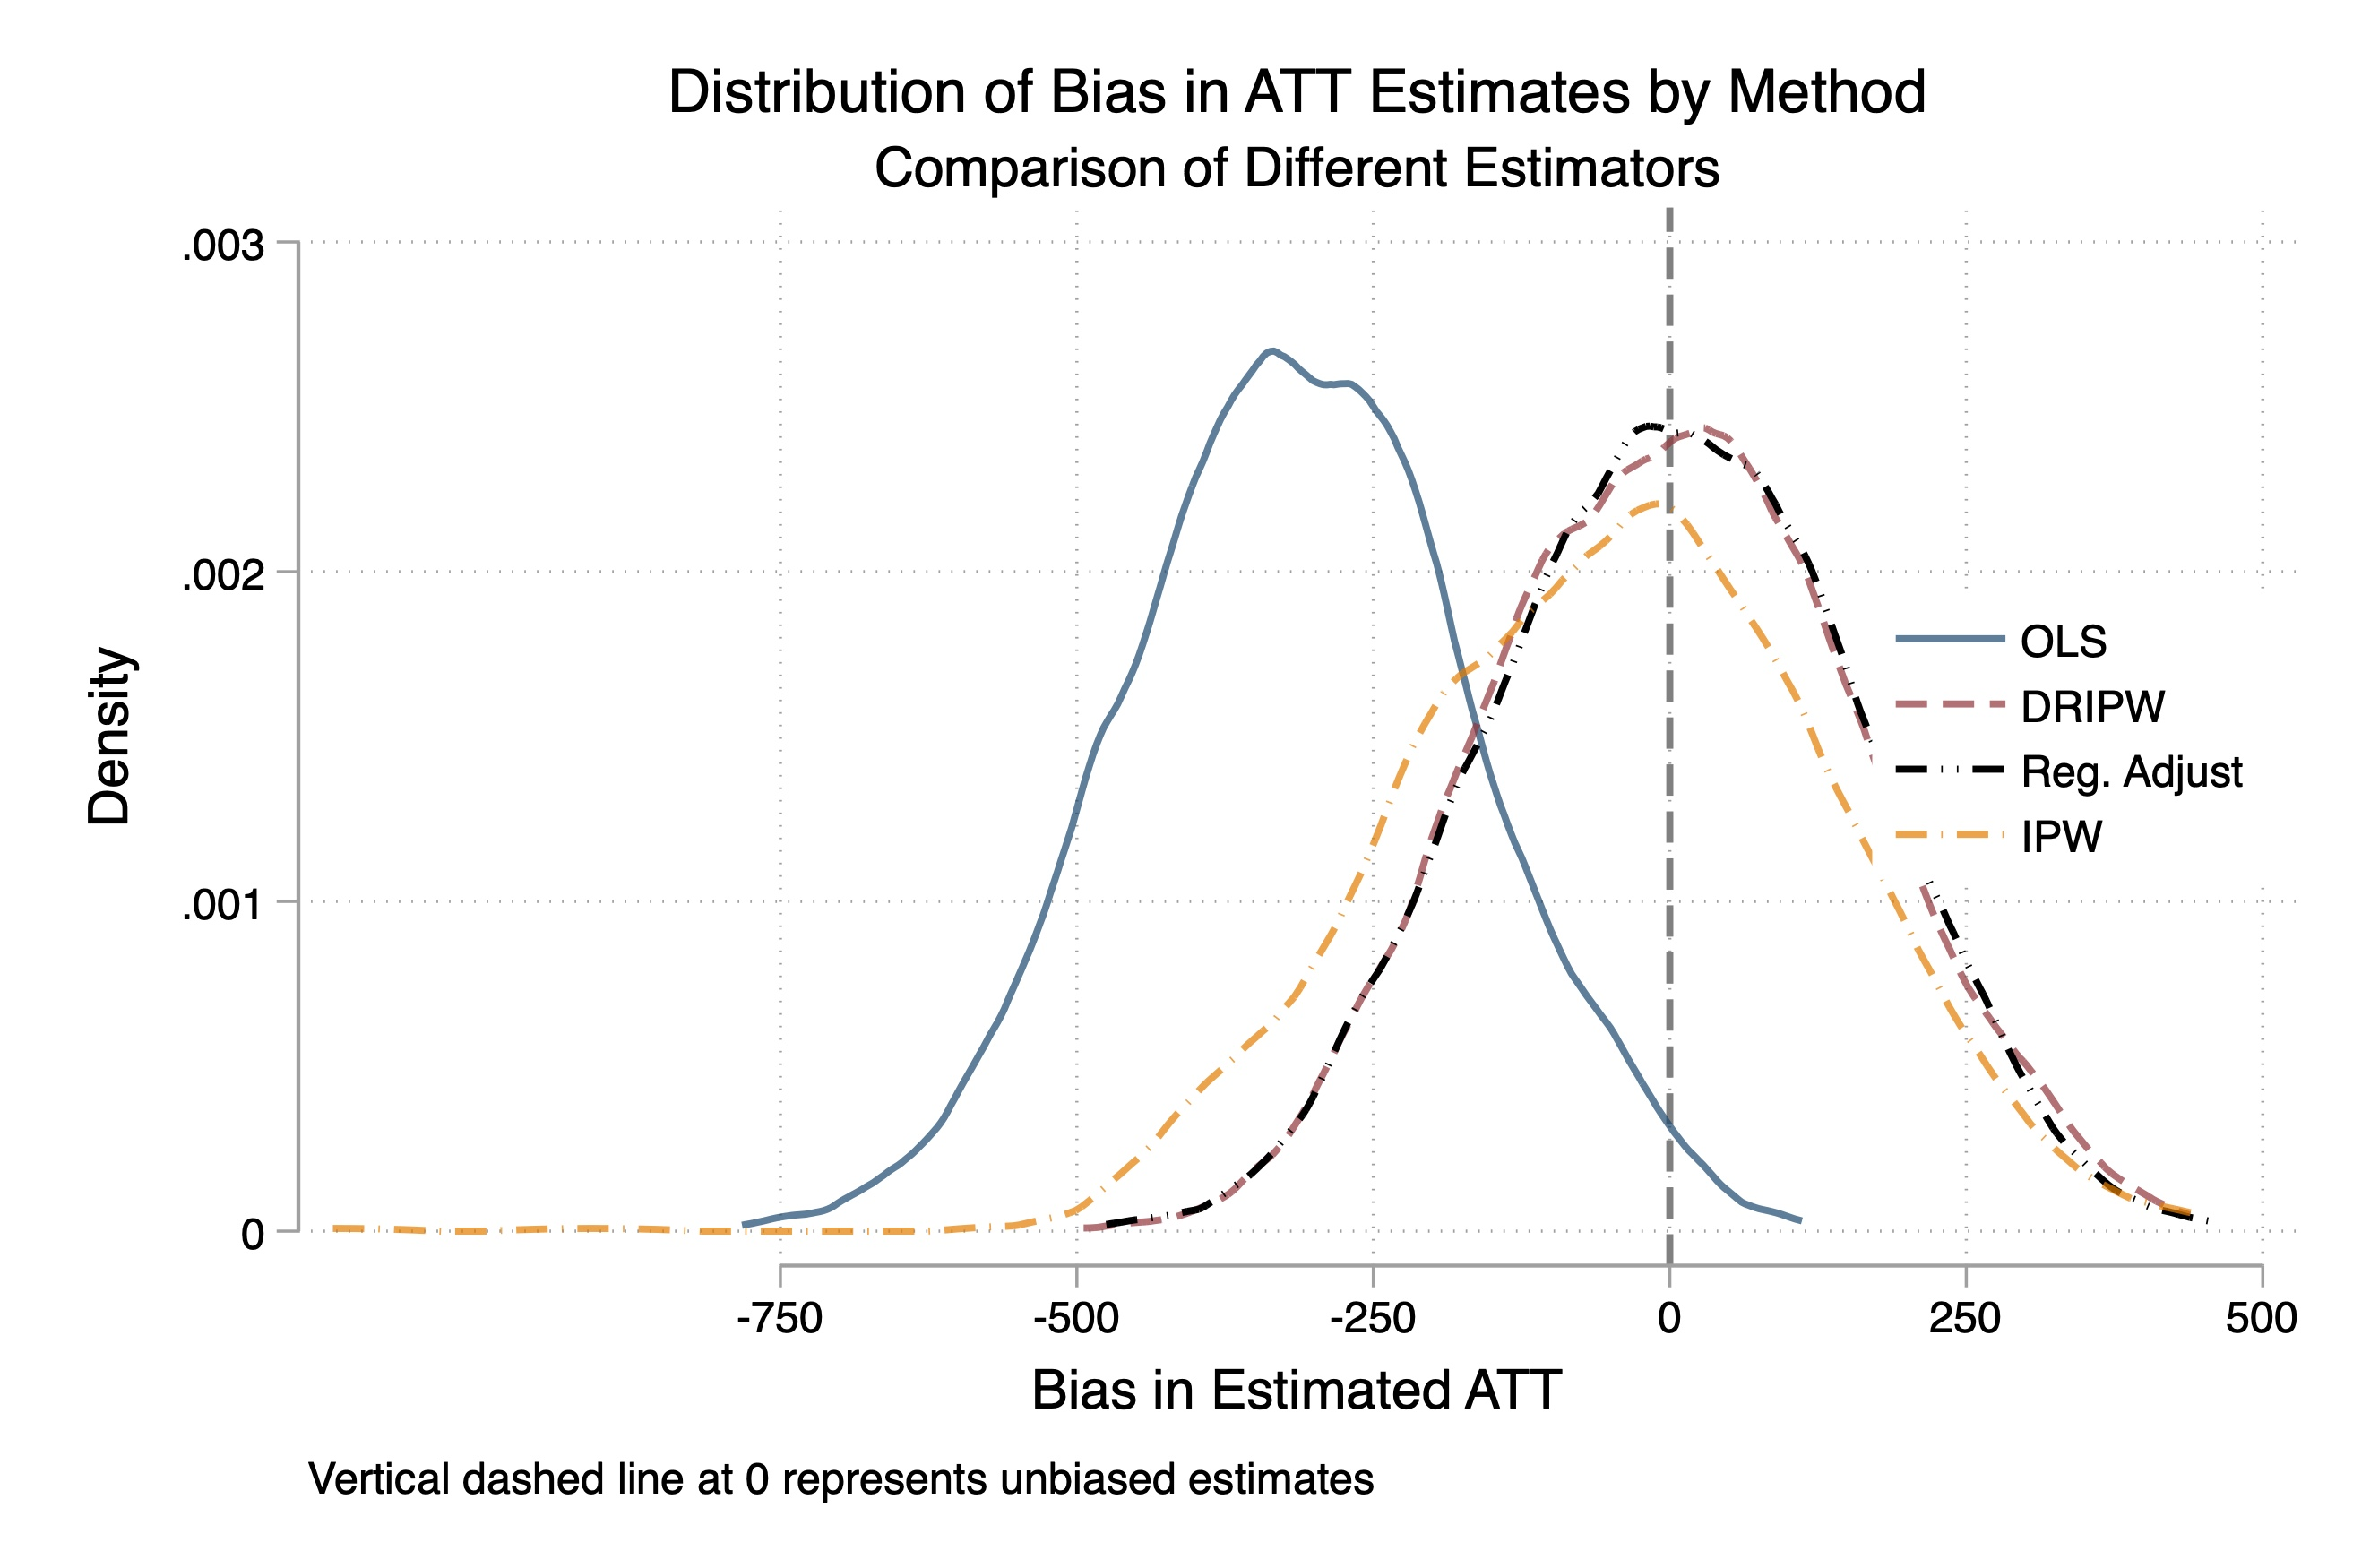
\includegraphics[width=0.6\textwidth]{./lecture_includes/covariates.jpg}
\end{frame}



\subsection{LaLonde dataset}

\begin{frame}{Application using real data}

\begin{itemize}
\item Let's now use a real example with real data and see how well this does
\item Famous paper in AER by Lalonde (1986), an Orley and Card student at Princeton
\item Found that most program evaluation did badly, but let's revisit it with diff-in-diff
\end{itemize}

\end{frame}

\begin{frame}{Description of NSW Job Trainings Program}
	
The National Supported Work Demonstration (NSW), operated by Manpower Demonstration Research Corp in the mid-1970s:
	\begin{itemize}
	\item was a temporary employment program designed to help disadvantaged workers lacking basic job skills move into the labor market by giving them work experience and counseling in a sheltered environment
	\item was also unique in that it \textbf{randomly assigned} qualified applicants to training positions:
		\begin{itemize}
		\item \textbf{Treatment group}: received all the benefits of NSW program
		\item \textbf{Control group}: left to fend for themselves
		\end{itemize}
	\item admitted AFDC females, ex-drug addicts, ex-criminal offenders, and high school dropouts of both sexes
	\end{itemize}
\end{frame}

\begin{frame}{NSW Program}
	
	\begin{itemize}
	\item Treatment group members were:
		\begin{itemize}
		\item guaranteed a job for 9-18 months depending on the target group and site
		\item divided into crews of 3-5 participants who worked together and met frequently with an NSW counselor to discuss grievances and performance
		\item paid for their work
		\end{itemize}
	\item Control group members were randomized so the same
	\item Note: the randomization balanced observables and unobservables across the two arms, thus enabling the estimation of an ATE for the people who self-selected into the program
	\end{itemize}
\end{frame}

\begin{frame}{NSW Program}

\begin{itemize}
	\item Other details about the NSW program:
		\begin{itemize}
		\item \underline{Wages}:  NSW offered the trainees lower wage rates than they would've received on a regular job, but allowed their earnings to increase for satisfactory performance and attendance
		\item \underline{Post-treatment}: after their term expired, they were forced to find regular employment
		\item \underline{Job types}:  varied within sites -- gas station attendant, working at a printer shop -- and males and females were frequently performing different kinds of work
		\end{itemize}
\end{itemize}

\end{frame}
	
\begin{frame}{NSW Data}
	
	\begin{itemize}
	\item \underline{NSW data collection}:
		\begin{itemize}
		\item MDRC collected earnings and demographic information from both treatment and control at baseline and every 9 months thereafter
		\item Conducted up to 4 post-baseline interviews
		\item Different sample sizes from study to study can be confusing, but has simple explanations
		\end{itemize}
	\end{itemize}
\end{frame}
	

\begin{frame}{NSW Data}

\begin{itemize}
	\item \underline{Estimation}:
		\begin{itemize}
		\item NSW was a randomized job trainings program; therefore estimating the average treatment effect is straightforward:
			\begin{eqnarray*}
			\frac{1}{N_t}\sum_{D_i=1}Y_i - \frac{1}{N_c}\sum_{D_i=0}Y_i \approx E[Y^1-Y^0] 
			\end{eqnarray*}in large samples assuming treatment selection is independent of potential outcomes (randomization) -- i.e., $(Y^0,Y^1)\independent{D}$. 
		\end{itemize}
	\item \underline{NSW worked}: Treatment group participants' real earnings post-treatment (1978) was positive and economically meaningful -- $\approx$ \$900 (LaLonde 1986) to \$1,800 (Dehejia and Wahba 2002) depending on the sample used
\end{itemize}

\end{frame}
	
\begin{frame}[plain]
	\begin{center}
	LaLonde, Robert J. (1986). \myurlshort{http://business.baylor.edu/scott_cunningham/teaching/lalonde-1986.pdf}{``Evaluating the Econometric Evaluations of Training Programs with Experimental Data''}. \emph{American Economic Review}. 
	\end{center}
	
\underline{LaLonde's study} was \textbf{not} an evaluation of the NSW program, as that had been done, but rather an evaluation of econometric models done by:
		\begin{itemize}
		\item replacing the experimental NSW control group with non-experimental control group drawn from two nationally representative survey datasets: Current Population Survey (CPS) and Panel Study of Income Dynamics (PSID)
		\item estimating the average effect using non-experimental workers as controls for the NSW trainees 
		\item comparing his non-experimental estimates to the experimental estimates of \$900
		\end{itemize}
\end{frame}

\begin{frame}{LaLonde (1986)}

\begin{itemize}

	\item \underline{LaLonde's conclusion}: available econometric approaches were biased and inconsistent
		\begin{itemize}
		\item His estimates were way off and usually the wrong sign
		\item Conclusion was influential in policy circles and led to greater push for more experimental evaluations
		\end{itemize}

\end{itemize}

\end{frame}

\imageframe{./lecture_includes/lalonde_table5a.png}
\imageframe{./lecture_includes/lalonde_table5b.png}

\begin{frame}[plain,shrink=10]{Imbalanced covariates for experimental and non-experimental samples}

    \begin{center}
		\begin{table}
		\begin{tabular}{lcccccc}
		\hline \hline
		\multicolumn{3}{c}{}&
		\multicolumn{1}{c}{CPS}&
		\multicolumn{1}{c}{NSW}\\
		
		\multicolumn{1}{c}{}&
		\multicolumn{2}{c}{All} &
		\multicolumn{1}{c}{Controls} &
		\multicolumn{1}{c}{Trainees} \\

		\multicolumn{3}{c}{}&
		\multicolumn{1}{c}{$N_c=15,992$}&
		\multicolumn{1}{c}{$N_t=297$}&
		\multicolumn{1}{c}{}&
		\multicolumn{1}{c}{}\\

		\multicolumn{1}{l}{covariate}&
		\multicolumn{1}{c}{mean}&
		\multicolumn{1}{c}{(s.d.)}&
		\multicolumn{1}{c}{mean}&
		\multicolumn{1}{c}{mean}&
		\multicolumn{1}{c}{t-stat}&
		\multicolumn{1}{c}{diff}\\
		\hline
Black    & 0.09 & 0.28 & 0.07 & 0.80 & 47.04 & -0.73\\
Hispanic & 0.07 & 0.26 & 0.07 & 0.94 & 1.47 & -0.02\\
Age & 33.07 & 11.04 & 33.2 & 24.63 & 13.37  & 8.6\\
Married & 0.70 & 0.46 & 0.71 & 0.17 & 20.54 & 0.54\\
No degree & 0.30 & 0.46 & 0.30 & 0.73 & 16.27 & -0.43\\
Education & 12.0 & 2.86 & 12.03 & 10.38 & 9.85 & 1.65 \\
1975 Earnings   & 13.51 & 9.31 & 13.65 & 3.1 & 19.63 & 10.6\\
1975 Unemp  & 0.11 & 0.32 & 0.11 & 0.37 & 14.29 & -0.26\\
		\hline 
		\end{tabular}
		\end{table}
    \end{center}

\end{frame}


\begin{frame}{Lab}

\url{https://github.com/Mixtape-Sessions/Causal-Inference-2/tree/main/Lab/Lalonde}

\bigskip

Together let's do questions 1 and 2a-c

\end{frame}


\section{Concluding Remarks}


\begin{frame}{Concluding remarks}

\begin{itemize}
\item Including covariates in a DiD design is done for reasons that are different than in regressions more generally -- we are trying to address a parallel trends violation
\item Typical regression modeling can only incorporate covariates, but that places restrictions on the model, whereas other methods will not
\item We use baseline covariates because we cannot include covariates that are outcomes otherwise it introduces its own biases
\item Doubly robust and IPW incorporate covariates through propensity scores and outcome regressions (or both) using baseline covariate means only
\end{itemize}

\end{frame}

\begin{frame}{Suggestions}

\begin{itemize}

\item Remember that the threat to validity comes from comparing aggregate groups of units for whom differences in observables, with different associations with $Y^0$, violate parallel trends
\item Conditional parallel trends simply requires that groups which are comparable on covariates are more likely to have comparable $Y^0$ trends
\item Check for imbalance at baseline using normalized differences
\item Choose covariates that are highly predictive of the missing potential outcome, $Y^0$

\end{itemize}

\end{frame}

\begin{frame}{Design stage}

\begin{itemize}

\item Keep in your mind that you are attempting to reassemble the dataset with the RCT metaphor in mind
\item Randomization distributes mean potential outcomes the same for treatment and control
\item We only need similar trends in $Y^0$ to be the same, and we think that's more likely within covariate strata
\item So, in the design stage, think carefully about this -- this is still prior to looking at the outcome data as this can inadvertently cause p-hacking
\item Remember -- you're the expert so use your knowledge of the phenomena to choose judiciously the covariates and be careful about causing the curse of dimensionality

\end{itemize}

\end{frame}

\end{document}
